32. $y=\cfrac{3-x}{|x^2-3x|}=\cfrac{3-x}{|x||x-3|}=\begin{cases} -\cfrac{1}{x},\ x>3,\\ \cfrac{1}{x},\ 0<x<3,\\ -\cfrac{1}{x},\ x<0. \end{cases}$
$$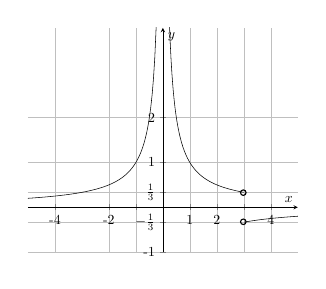
\begin{tikzpicture}[scale=0.5]
\begin{axis}[
    axis lines = middle,
    grid=major,
    legend pos={south west},
    xlabel = {$x$},
    %xlabel style={below right},
    ylabel = {$y$},
    ymin=-1,
    ymax=4,
    xtick={-4, -2,-1,1, 2,3,4},
    xticklabels={-4, -2,$ $, 1, 2,$ $, 4},
    ytick={-2,-1,-0.33,0.33, 1, 2},
     yticklabels={-2,-1,$-\frac{1}{3}$,$\frac{1}{3}$, 1, 2},
                  ]
	\addplot[domain=-5:-0.1, samples=100, color=black] {-1/x};
    \addplot[domain=0.1:2.99, samples=100, color=black] {1/x};
    \addplot[domain=3.01:5, samples=100, color=black] {-1/x};
   % \addplot[domain=1.01:5, samples=100, color=black] {3/(x+1)};
    %\addlegendentry{$\text{Рис. 1}$};
\end{axis}
\draw (5.47,1.51) circle (2pt);
\draw (5.47,0.77) circle (2pt);
\end{tikzpicture}$$
